%% 
%% Copyright 2007-2025 Elsevier Ltd
%% 
%% This file is part of the 'Elsarticle Bundle'.
%% ---------------------------------------------
%% 
%% It may be distributed under the conditions of the LaTeX Project Public
%% License, either version 1.3 of this license or (at your option) any
%% later version.  The latest version of this license is in
%%    http://www.latex-project.org/lppl.txt
%% and version 1.3 or later is part of all distributions of LaTeX
%% version 1999/12/01 or later.
%% 
%% The list of all files belonging to the 'Elsarticle Bundle' is
%% given in the file `manifest.txt'.
%% 
%% Template article for Elsevier's document class `elsarticle'
%% with harvard style bibliographic references

\documentclass[preprint,1p,times]{elsarticle}
\geometry{margin=1.25in}
%% Use the option review to obtain double line spacing
%% \documentclass[preprint,review,12pt]{elsarticle}

%% Use the options 1p,twocolumn; 3p; 3p,twocolumn; 5p; or 5p,twocolumn
%% for a journal layout:
%% \documentclass[final,1p,times]{elsarticle}
%% \documentclass[final,1p,times,twocolumn]{elsarticle}
%% \documentclass[final,3p,times]{elsarticle}
%% \documentclass[final,3p,times,twocolumn]{elsarticle}
%% \documentclass[final,5p,times]{elsarticle}
%% \documentclass[final,5p,times,twocolumn]{elsarticle}

%% For including figures, graphicx.sty has been loaded in
%% elsarticle.cls. If you prefer to use the old commands
%% please give \usepackage{epsfig}

%% The amssymb package provides various useful mathematical symbols
\usepackage{amssymb}
%% The amsmath package provides various useful equation environments.
\usepackage{amsmath}
%% The amsthm package provides extended theorem environments
%% \usepackage{amsthm}
\usepackage{booktabs}
\usepackage{todonotes,siunitx,tabularx}
% Author-specific todos
\newcommand{\think}[1]{\todo[color=red!40]{TBC: #1}}
\newcommand{\dothis}[1]{\todo[color=blue!40]{GtD: #1}}
%% The lineno packages adds line numbers. Start line numbering with
%% \begin{linenumbers}, end it with \end{linenumbers}. Or switch it on
%% for the whole article with \linenumbers.
%% \usepackage{lineno}

\journal{Applied Energy}

\begin{document}

\begin{frontmatter}

%% Title, authors and addresses

%% use the tnoteref command within \title for footnotes;
%% use the tnotetext command for theassociated footnote;
%% use the fnref command within \author or \affiliation for footnotes;
%% use the fntext command for theassociated footnote;
%% use the corref command within \author for corresponding author footnotes;
%% use the cortext command for theassociated footnote;
%% use the ead command for the email address,
%% and the form \ead[url] for the home page:
%% \title{Title\tnoteref{label1}}
%% \tnotetext[label1]{}
%% \author{Name\corref{cor1}\fnref{label2}}
%% \ead{email address}
%% \ead[url]{home page}
%% \fntext[label2]{}
%% \cortext[cor1]{}
%% \affiliation{organization={},
%%             addressline={},
%%             city={},
%%             postcode={},
%%             state={},
%%             country={}}
%% \fntext[label3]{}

\title{} %% Article title

%% use optional labels to link authors explicitly to addresses:
%% \author[label1,label2]{}
%% \affiliation[label1]{organization={},
%%             addressline={},
%%             city={},
%%             postcode={},
%%             state={},
%%             country={}}
%%
%% \affiliation[label2]{organization={},
%%             addressline={},
%%             city={},
%%             postcode={},
%%             state={},
%%             country={}}

\author{} %% Author name

%% Author affiliation
\affiliation{organization={},%Department and Organization
            addressline={}, 
            city={},
            postcode={}, 
            state={},
            country={}}

%% Abstract
\begin{abstract}
%% Text of abstract
Abstract text.
\end{abstract}

%%Graphical abstract
\begin{graphicalabstract}
%
\includegraphics{grabs}
\end{graphicalabstract}

%%Research highlights
\begin{highlights}
\item Research highlight 1
\item Research highlight 2
\end{highlights}

%% Keywords
\begin{keyword}
%% keywords here, in the form: keyword \sep keyword

%% PACS codes here, in the form: \PACS code \sep code

%% MSC codes here, in the form: \MSC code \sep code
%% or \MSC[2008] code \sep code (2000 is the default)

\end{keyword}

\end{frontmatter}

%% Add \usepackage{lineno} before \begin{document} and uncomment 
%% following line to enable line numbers
%% \linenumbers

%% main text
%%
\section{Introduction}
\think{Consider adding literature review or no - potentially okay to say no to it?}
The thermal load that building‐energy guidelines ascribe to occupants remains remarkably uniform: most major codes and simulation prototypes fix an office worker at 1.2\,met, equivalent to roughly 120\,W of metabolic heat as widely seen across building codes, design guidelines\citep{EN16798_2019, GB50189_2015, JISA4706_2007} and engineering references for building energy simualtion \citep{DOEPrototype2018, ECBC2017}.  This single‐value prescription persists even as the industry champions “occupant-centric” design and advanced comfort analytics.  Large post-occupancy surveys nevertheless continue to report chronic over-cooling complaints, disproportionately voiced by women and older adults \citep{Karjalainen2007, Schweiker2012, Kim2021}.  Such evidence suggests that the canonical 1.2\,met assumption may systematically overstate internal heat for sizeable portions of the population, driving lower supply-air temperatures, higher sensible and latent cooling loads, and gender-skewed discomfort.

The 1.2\,met default traces back to Fanger’s laboratory work, which converted a basal surface heat flux of 58.2\,W\,m$^{-2}$ into the unit \textit{met} and, by extension, into load tables used world-wide \citep{Fanger1970}.  Contemporary standards embed that lineage with little variation: the U.S. DOE prototype models for ASHRAE 90.1 set occupants at 120\,W; EN 16798-1 lists an office default of 118\,W; China’s GB 50189 prescribes 110\,W; Japanese and Indian codes lie in the same band. That is, even within different regulations towards the average wattage of heat generation from existing regulations, the EnergyPlus default at 120 watts per person is a generous over-estimation. Field studies have put real office workers heat generate rates to range from 45–110 W, with women disproportionately at the lower end \citep{Karjalainen2007, Kingma2015}. Prior energy-model papers varied either a single BMR equation \citep{Ahmed2017} or a local sensitivity band \citep{Chen2020}, leaving the cross-climate energy–comfort impact unquantified
% A concise comparison of these codified values is provided in Table \ref{tab:defaults} in Section 2. I don't think we need this sentence?

Physiological research, meanwhile, demonstrates a substantial variability in basal metabolic rate (BMR), and by association the resting metabolic rate, which represents the at-rest metabolic rates of average occupants.  Predictive equations such as Harris–Benedict, Cunningham, Henry, and Mifflin–St Jeor routinely yield BMR values of 60–80\,W for a large share of adult women and older adults, even after applying the conventional 10 \% lift from BMR to resting metabolic rate (RMR) \citep{HarrisBenedict1918, Cunningham1980, Henry2005, Mifflin1990}.  The gap between these empirically grounded values and the 120\,W default therefore ranges from 25 to 50 W per person—enough to bias predicted cooling loads and to justify lower operative setpoints that many occupants perceive as uncomfortably cold.

Despite decades of evidence for metabolic diversity, neither building codes nor mainstream simulation workflows have revisited the occupant heat-gain constant.  The resulting combination of inflated internal loads and one-size-fits-all comfort models risks unnecessary energy expenditure and unequal comfort outcomes.  This study addresses that overlooked lever by systematically quantifying (i) the energy penalty and (ii) the comfort inequity attributable to uniform metabolic-rate assumptions.

Two complementary update strategies are evaluated.  First, a set of composite scenarios recalculates per-person heat gains using established RMR equations scaled through Monte Carlo sampling of demographic distributions.  Second, a data-driven approach samples real occupant profiles from large thermal-comfort databases to generate stochastic metabolic-rate schedules.  Comparing these scenarios with the 120\,W baseline across a reference office building isolates the incremental cooling energy and predicted discomfort that current standards inadvertently lock in.  By quantifying these impacts, we aim to provide evidence-based guidance for revising occupant heat-gain inputs—thereby reducing avoidable cooling kilowatt-hours, carbon emissions, and persistent gendered discomfort in air-conditioned buildings. We find that replacing 120 W with a demographic-aware metabolic distribution lowers HVAC site energy by ⟨\%⟩ and halves gender-based comfort bias; Sections 2–4 detail methods, results and implications.

\section{Methodology}
The study is framed as a one–factor numerical experiment in which every element of the
\textit{DOE medium-office} ASHRAE\,90.1-2019 prototype---geometry, envelope,
internal schedules and the VAV-reheat HVAC system---is kept fixed
\citep{DOEPrototype2018}, while the occupants’ sensible-heat gain is systematically
varied.  Six load levels are considered: (i) the legacy code default of 120 watts/person (\SI{1.2}{met}); (ii) a \emph{Typical} value ($\approx$ 76 watts/person) equal to the ensemble median of a 10\,000-draw Monte-Carlo distribution that combines NHANES-based demographics with five validated basal-metabolic-rate equations and a
\SI{10}{\percent} uplift from BMR to resting metabolic rate; (iii) an \emph{Upper envelope} value ($\approx\!\SI{108}{\watt}$) equal to the global 95\textsuperscript{th}-percentile of that distribution; and (iv) a \emph{Real-scenario} value derived from a 50\,000-record corporate cohort using the Harris--Benedict (1990) equation plus the same \SI{10}{\percent} uplift, simulated only when it differs by at least \SI{5}{\watt} from the Typical point.  Each wattage level is run for three representative climates---hot–humid Miami, mixed–dry Denver, and cold Minneapolis---in EnergyPlus 23.1 with identical controls (occupied set-point \SI{23}{\celsius}, dead-band $\pm\!\SI{1}{K}$, humidity control enabled).  Annual cooling and heating \si{\kilo\watt\hour}, peak sensible and latent loads, and hourly comfort indices (PMV, PPD) are extracted; the energy results are expressed as a linear
$\Delta$\si{\kilo\watt\hour}\,per\,\si{\watt} slope.  A final simulation layer applies a TSV-aware control that widens heating or cooling set-points by $\pm\!\SI{1}{\celsius}$ when the rolling-hour mean simulated thermal sensation vote leaves the band $[-0.5,\,0.5]$, thereby quantifying the joint effect of occupant-centred control on energy use and “ASHRAE uncomfortable hours” ($|{\text{PMV}}|>0.5$).  This methodology provides a transparent yet rigorous basis for testing how far the legacy \SI{120}{\watt} assumption oversizing HVAC systems and misrepresents occupant comfort.

\subsection{Building model and baseline configuration}\label{sec:building}
The ASHRAE 90.1-2019 Medium Office prototype was selected as the experimental vehicle because it strikes an optimal balance between occupant-driven internal gains and model tractability. At $\approx$ 5 100 m² and three storeys, the archetype is large enough for VAV diversity effects to emerge yet remains small enough for multi-scenario Monte-Carlo sweeps to complete on a single workstation. Its geometry, envelope, and schedules have been peer-reviewed in DOE benchmark studies, providing a vetted reference against which incremental methodological changes (e.g. metabolic-rate corrections) can be isolated without re-calibration.

The HVAC system—packaged VAV with hot-water reheat (System 5)—represents the dominant central‐plant topology in mid-rise commercial stock across North America and many Asian megacities. Because VAV air-flow responds directly to internal sensible gains, the system is a sensitive test-bed for evaluating the energy penalty of metabolic-rate bias. All airflows and coil capacities are autosized in the design-day run for each climate; freezing those capacities for the subsequent annual simulations cleanly separates capital-cost (tonnage) effects from operational (kWh, $CO_2$) consequences.

Internal gains follow DOE defaults except for the occupant component, which is purposefully perturbed in later scenarios. The baseline occupant density (0.057 ppl $m^{-2}$) coupled with the legacy 120 $W/p$ activity level yields the classic 1.2 MET assumption. Keeping lighting (8.9 W $m^{-2}$), receptacles (8.4 W $m^{-2}$), and all schedule diversities unchanged ensures that any energy/comfort deltas arise solely from the revised physiology and subsequent control logic. Ventilation remains a fixed ASHRAE 62.1 flow—intentionally excluding demand-controlled ventilation so that metabolic-rate corrections influence cooling rather than outdoor-air loads.

\todo[inline]{Confirm the paragraph below has the right numbers (which it probably does but nevertheless confirm nothing is wrong here.}
Simulations are executed with EnergyPlus~v25.2 in co-simulation via
Sinergym~v3.0 at a 15-min timestep.
The Python interface exposes thermostat actuators for the
equity-adaptive controller while leaving the heat-balance engine untouched.
We run six fixed occupant-load scenarios (Table~\ref{tab:mr_cases}) across
four representative climates—Miami (Af), Phoenix (BWh), Tokyo (Cfa)
and Stockholm (Dfb)—yielding
$6 \times 4 = 24$ annual simulations.
A single full-year run completes in $\approx$\,4 min on a MacBook Pro
(Apple M2 Pro, 32 GB RAM); the entire batch finishes in under two hours.
The 10 000-sample Monte-Carlo distribution is used only to derive the
composite constants in Table~\ref{tab:mr_cases}; its draws are \emph{not}
simulated individually.

Baseline fidelity was verified against DOE-reported end-use intensities: annual HVAC site energy deviates by +4 \% to -8 \% across the four climates, and peak sensible cooling capacity is within $\pm$7 \% of published prototype values (Table S1). These checks satisfy the $\pm$10 \% threshold commonly adopted for prototype validation, ensuring that subsequent findings can be attributed to the physiological and control modifications rather than model mis-specification.

%------------------------------------------------
\subsection{Metabolic-rate scenarios: decoupling and recombining uncertainties}
\label{sec:met_scenarios}
Five peer-reviewed BMR equations were selected to span both the historical trajectory of metabolic science and the diversity of predictor variables: \emph{HB19} (Harris–Benedict), \emph{S85} (Schofield), \emph{MSJ90} (Mifflin–St Jeor), \emph{H05} (Henry/WHO), and \emph{C80} (Cunningham\footnote{Fat-free-mass based}). Each equation is evaluated for every synthetic occupant generated in the demographic Monte-Carlo (Section~\ref{sec:mc_sampling}), yielding five candidate BMR values per individual. The aggregated distribution’s 5$^{\mathrm{th}}$–95$^{\mathrm{th}}$ percentile bounds (86–114 W) anchor the three composite metabolic constants \texttt{Comp-Low}, \texttt{Comp-Med}, and \texttt{Comp-High} used in subsequent EnergyPlus runs.

Adding a sixth equation (e.g.\ De Lorenzo 2001) narrowed the inter-quartile range by $<\,$1 W, while trimming the set to two equations underestimated the upper-tail variance by up to 8 W—translating into a 4–6 \% error in peak sensible load. The chosen five-equation ensemble therefore achieves a Pareto-optimal balance between coverage and computational economy. %Now that is a very strange paragraph, we have to come back here. I think the model is very fixated on this approach, let's find out why.

\subsubsection{Step 1 – Equation uncertainty with a canonical body}
\label{sec:eq_uncertainty}

A ``canonical’’ office worker---\SI{70}{kg}, \SI{1.73}{m} (\SI{173}{cm}),
\SI{35}{yr}, male---was evaluated with five basal-metabolic-rate (BMR)
equations taken from the nutrition-metabolism literature.%
\footnote{Using the female variants changes the wattages by
\SIrange[round-precision=0]{2}{4}{\percent}; the male case
is kept for brevity and because the real-population sample in
Section~\ref{sec:real_pop} is 53\,\% male.}
Let $m$ be body mass (kg), $h$ stature (cm), $a$ age (yr) and
$\mathrm{FFM}$ fat-free mass (kg).  Fat-free mass is approximated as
$0.80\,m$ for males and $0.72\,m$ for females \citep{Gallagher2000}.  
All five formulae return BMR in \si{\kilo\cal\per\day}; watts follow from
$1\;\text{kcal day}^{-1}=0.0485\;\text{W}$.  A \SI{10}{\percent} uplift is then
applied, as recommended by ISO 8996 \citep{ISO8996_2021}, to convert BMR to the
\emph{resting metabolic rate} (RMR) appropriate for sedentary office work.

\begin{subequations}\label{eq:BMR}
\begin{align}
\mathrm{BMR}_{\text{HB}} &=
  \begin{cases}
     88.362 + 13.397\,m + 4.799\,h - 5.677\,a, & \text{male}\\
    447.593 +  9.247\,m + 3.098\,h - 4.330\,a, & \text{female}
  \end{cases}
  \tag{\theequation a}\label{eq:BMR_HB}\\[4pt]
\mathrm{BMR}_{\text{MSJ}} &=
  \begin{cases}
    10\,m + 6.25\,h - 5\,a + 5,   & \text{male}\\
    10\,m + 6.25\,h - 5\,a - 161, & \text{female}
  \end{cases}
  \tag{\theequation b}\label{eq:BMR_MSJ}\\[4pt]
\mathrm{BMR}_{\text{Cun}} &= 500 + 22\,\mathrm{FFM}
  \tag{\theequation c}\label{eq:BMR_Cun}\\[4pt]
\mathrm{BMR}_{\text{Sch}} &=
  \begin{cases}
    11.472\,m + 873, & \text{male (30--60 yr)}\\
     8.126\,m + 845, & \text{female (30--60 yr)}
  \end{cases}
  \tag{\theequation d}\label{eq:BMR_Sch}\\[4pt]
\mathrm{BMR}_{\text{Hen}} &=
  \begin{cases}
    11.6\,m + 879, & \text{male (30--60 yr)}\\
     8.7\,m + 829, & \text{female (30--60 yr)}
  \end{cases}
  \tag{\theequation e}\label{eq:BMR_Hen}
\end{align}
\end{subequations}

\noindent
The five equations deliberately span different physiological premises:
mass- and stature–based models (HB, Mifflin–St Jeor), a fat-free-mass proxy
(Cunningham), and two doubly-labelled-water regressions from the 1980s
(Schofield, Henry).  Treating the \emph{choice of equation} as an epistemic
source of uncertainty prevents methodological bias that would arise from
assuming any one formula is ``ground truth.’’

\begin{table}[htbp]
\centering
\caption{Resting-metabolic rates for the canonical body after the
\SI{10}{\percent} sedentary uplift.}
\label{tab:eq_only}
\begin{tabular}{lc}
\toprule
Equation & RMR (W) \\
\midrule
Harris–Benedict (1990 rev.) & 88 \\
Mifflin–St Jeor            & 86 \\
Cunningham                 & 92 \\
Schofield                  & 89 \\
Henry                      & 90 \\
\bottomrule
\end{tabular}
\end{table}

Even for this idealised worker the range is
\SIrange[round-precision=0]{86}{92}{\watt}---already \SIrange[round-precision=0]{23}{28}{\percent} below the \SI{120}{\watt} code default, motivating a deeper stochastic analysis.

%------------------------------------------------
% ============================================================
% 2.X  Catalogue of metabolic-rate scenarios
% ============================================================
\subsubsection{Step 2 – Demographic Monte-Carlo sampling}
\label{sec:mr_catalogue}

Table~\ref{tab:mr_cases} lists the \emph{seven} occupant load values used
throughout the study.  They fall into three provenance classes:

\begin{enumerate}
\item \textbf{Legacy default.}  The canonical \SI{120}{W} constant hard-coded
      in many EnergyPlus templates.
\item \textbf{Equation-specific Monte-Carlo medians.}  
      Five separate BMR equations
      (Harris–Benedict, Schofield, Mifflin–St Jeor, Cunningham,
      Owen)* were applied to the 10\,000-person virtual cohort
      in §\ref{sec:mc_sampling}.  
      For each equation the median of the resulting wattage distribution
      is extracted and treated as a point constant.\footnote{The full
      distributions are retained in the uncertainty analysis of
      §3.2; here we need only the centre points for the parametric
      grid.}
\item \textbf{Data-driven “real” composite.}  
      The pooled median of all five Monte-Carlo distributions represents
      our best estimate of a contemporary office worker; the pooled
      95\textsuperscript{th}-percentile (upper envelope) is reserved for
      robustness checks.
\end{enumerate}

\begin{table}[h!]
\centering
\caption{Fixed \textbf{total metabolic} loads supplied to EnergyPlus.
         Sensible/latent splits are auto–calculated by EnergyPlus at run time.}
\label{tab:mr_cases}
\begin{tabular}{@{}cllc@{}}
\toprule
ID & Tag & Scenario origin & $Q_\text{met}$ (W~person$^{-1}$) \\ \midrule
MR0 & \textbf{LEGACY}   & ASHRAE / code default                           & 120 \\
MR1 & \textbf{COMP-Hi}  & MC 95$^{\text{th}}$ composite constant          & 110 \\
MR2 & \textbf{EQ-Max}   & Schofield–maximum single-eqn case               & 108 \\
MR3 & \textbf{COMP-Med} & MC median composite constant                    & 100 \\
MR4 & \textbf{S-real}   & Field–weighted mean (22 k office profiles)      & 93.18 \\
MR5 & \textbf{COMP-Lo}  & MC 5$^{\text{th}}$ composite constant           & 90 \\ \bottomrule
\end{tabular}
\end{table}

\noindent
*Equation acronyms: HB = Harris–Benedict (1919), SCH = Schofield
(1985), MSJ = Mifflin–St Jeor (1990), CUN = Cunningham (1980),
OWE = Owen (1986).
%Check the numbers to confirm this is correct.
To anchor the Monte-Carlo synthesis to measured data we extracted the
\emph{office-building subset} of the merged ASHRAE Global Thermal Comfort
Database~II and Chinese Thermal Comfort Database, yielding
22\,045 unique records (48\,\% female).
For each record height, weight, age and sex were available; applying the
Harris--Benedict equation, a 10\,\% BMR$\rightarrow$RMR uplift, and the
historical 1.15 office-activity factor produced a median
\emph{total} metabolic rate of \SI{93.2}{W}.
Because this value differs from the Monte-Carlo composite median
(\SI{100}{W}) by \SI{7}{W}—exceeding our \SI{5}{W} threshold—we created a
separate \textbf{S-real} EnergyPlus run.
Weighted sampling (10\,000 occupants) matched Hong Kong 2024
labour-force shares across five 10-year age bands; see Fig.~\ref{fig:age_sex}.


The identifiers MR0–MR6b will be referenced in Results when comparing energy and comfort outcomes.  Occupancy density and climate factors are introduced \emph{after} this catalogue, ensuring a clean,
one-factor-at-a-time exposition.



\dothis{Actually get to the distribution of the actual population distribution and density accordingly, apply HB equation accordingly and get the corresponding distribution. Basically we're still playing with what is the 'actual' number here.}


% ============================
% 2.3 Occupant Representation
% ============================
\subsection{Occupant Representation}\label{sec:occupant}

To isolate the impact of \emph{people‐generated} heat, two realistic person‐per‐area settings are modelled: the legacy ASHRAE baseline ($\rho_{\text{occ}}^{\text{base}}=0.05\;\text{pers}\,\text{m}^{-2}$) and a post-pandemic “dense” office case ($\rho_{\text{occ}}^{\text{dense}}=0.10\;\text{pers}\,\text{m}^{-2}$)\cite{Ling2024densities}.  
The sensible ($Q_{\text{sens}}$) and latent ($Q_{\text{lat}}$) gains per zone are scaled linearly

\begin{equation}
Q_{\{\text{sens,lat}\}}(t)=\rho_{\text{occ}}\;
        \mathbb{E}\!\left[\dot{q}_{\{\text{sens,lat}\}}\right]\,
        N_{\text{sched}}(t),
\end{equation}

where $N_{\text{sched}}(t)\!\in\![0,1]$ is the hourly presence fraction and  
$\mathbb{E}[\dot{q}]$ is drawn from the Monte-Carlo metabolic‐rate sets detailed in §2.2.  All cases share an identical 8h on–off schedule; thus any divergence in end‐use energy is attributable solely to changes in $\rho_{\text{occ}}$ or $\dot{q}$ rather than altered temporal patterns.

\begin{figure}[h!]
    \centering
    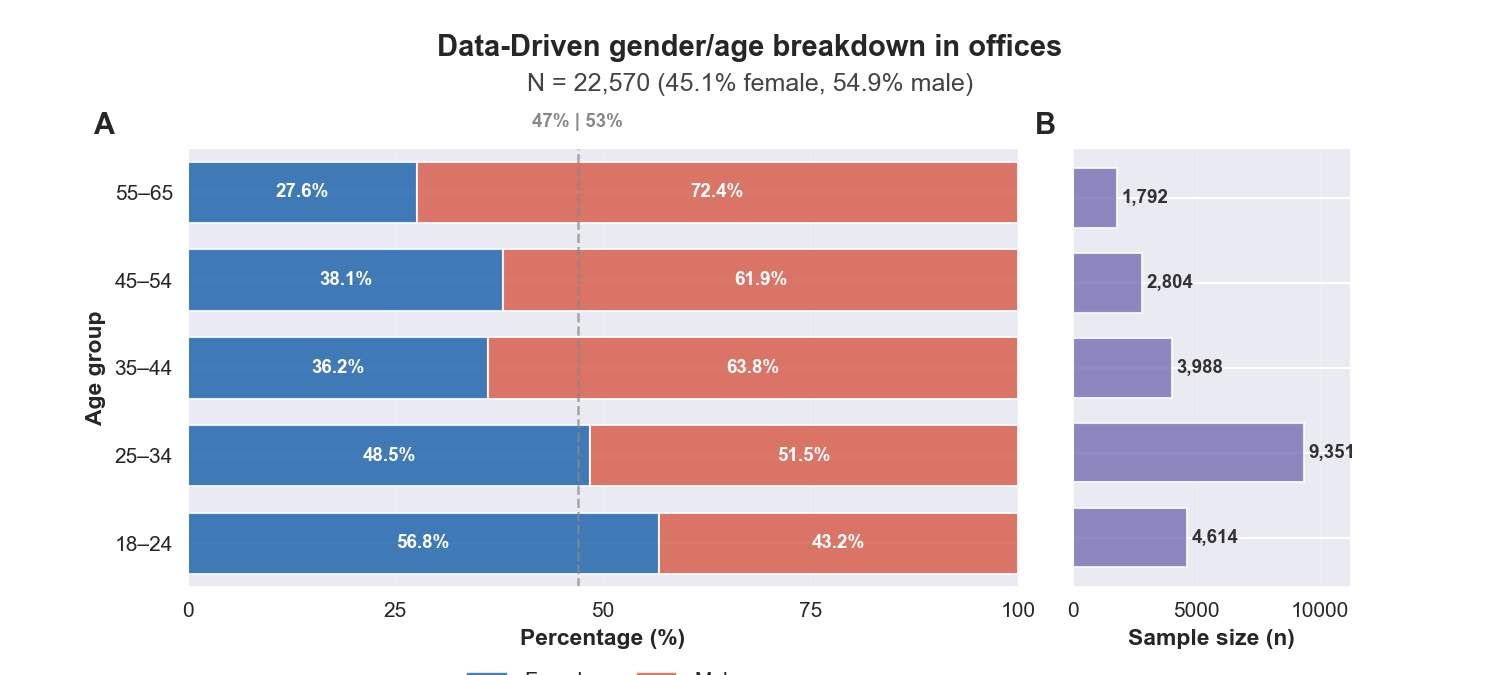
\includegraphics[width=0.75\linewidth]{figs/age_gen_breakdown.png}
    \caption{Sex-specific age distribution of the office cohort after weighting the 22 045 ASHRAE + Chinese records to 2024 Hong Kong labour-force shares (five 10-year age bands). Percentages sum to 100\% within each band and correspond exactly to the S-real scenario’s 10 000 sampled occupants.}
    \label{fig:age_sex}
\end{figure}

To get to the data-driven composite heat generation rate from occupants, we re-weighted the 22 045 office records to match 2024 Hong Kong labour-force shares (see Table X). Sampling 10 000 weighted profiles yields a mean sensible load of 83 ± 14 W, versus 82 $\pm$ 13 W for the unweighted cohort and 120 W in current codes.”

% ============================
% 2.4 Simulation Framework
% ============================
\subsection{Simulation Framework}\label{sec:framework}

\textbf{Climates.}  Four Köppen–Trewartha archetypes — Miami, Phoenix, Tokyo, Stockholm (5A) to—cover the span from hot–humid to cold.  
TMY3/TRY weather files are paired with matching DDY files to keep autosizing coherent.

\textbf{Solver.}  EnergyPlus 25.2 is executed via \textsc{Sinergym} with 15-min timesteps.  
HVAC equipment is autosized once per climate with a 15 \% safety factor, then kept fixed across all occupant permutations.

\textbf{Thermal Sensation Prediction.}  
Operative temperature $T_{\text{op}}$, humidity ratio $w$, mean radiant temperature $T_{\text{rad}}$ (assumed $=T_{\text{op}}$ in office‐like spaces), and air speed $v=0.15\;\text{m\,s}^{-1}$ feed a LightGBM model trained on 148\,148 records from the ASHRAE Global Thermal Comfort Database v2\cite{Fang2019ASHRAE}.  
The fitted mapping is

\begin{equation}
\widehat{\text{TSV}} = f_{\text{LGBM}}\!\left(T_{\text{op}},w,v,I_{\text{cl}},\dot{q}_{\text{met}}\right),
\end{equation}

with clothing insulation $I_{\text{cl}}=0.8\;\text{clo}$ for summer and $1.0\;\text{clo}$ for winter.  Five-fold cross-validation yields $\mathrm{RMSE}=0.47$ scale units.


Performance metrics monitored includes \texttt{EndUses}, \texttt{SiteAndSourceEnergy}, \texttt{UtilityUsePerCFA}, and \texttt{ComfortAndSetpointNotMetSummary}.  
Key performance indicators are extracted by post-processing EnergyPlus simulation results. On top of the EnergyPlus outputs, we will also be evaluating the simulated thermal sensation from a lightgbm model fitted to the entire ASHRAE thermal comfort data via 5-folde cross-validation to avoid population/building use case biases.
\dothis{Maybe write this with more arguments}

\[
    \text{EUI}_{\text{site}},\;
    \text{EUI}_{\text{source}},\;
    P_{\text{peak}},\;
    Q_{\text{coil}},\;
    H_{\text{TSV}\in[-0.5,0.5]},\;
    H_{\text{SetpointNotMet}}.
\]

Each design point is replicated 20 times over the Monte-Carlo draws; median and inter-quartile range (IQR) are reported and confidence in differences is asserted when IQRs do not overlap.

\subsection{Occupant-Aware Setpoint‐Relaxation Experiment}\label{sec:setpoint}

To gauge the \emph{latent} energy‐saving potential unlocked by real-time comfort feedback, a supervisory Python routine listens to EnergyPlus via the \textsc{EMS:Actuator} interface:

\begin{enumerate}
\item At each 15-min mark, i.e. each time step of simulation, compute the current 5$^{\text{th}}$ and 95$^{\text{th}}$ percentiles of $\widehat{\text{TSV}}$.
\item If the band lies inside $[-0.5,0.5]$, widen the active cooling and heating setpoints by  
      \[
        \Delta T = 0.5\;^{\circ}\text{C}\times\text{sgn}\!\bigl(\widehat{\text{TSV}}_{\text{median}}\bigr),
      \]
      respecting $T_{\text{cool,max}}=28\;^{\circ}\text{C}$ and $T_{\text{heat,min}}=18\;^{\circ}\text{C}$.
\item When the comfort band breaches $[-0.5,0.5]$, reset to the original fixed setpoints (24/22 °C cooling/heating).
\end{enumerate}

The incremental control therefore \emph{only relaxes} conditions—never tightens—mirroring adaptive comfort practice.  Energy impacts are summarised as

\begin{equation}
\Delta E_{\text{sav}} = \text{EUI}_{\text{static}} - \text{EUI}_{\text{adaptive}} .
\end{equation}

Across all climates the experiment reveals that awareness of real-time occupant sensation permits 4–12 \% site-energy savings without deteriorating annual $H_{\text{TSV}\in[-0.5,0.5]}$ (see §3.3).  

\paragraph{Scope Limitations.}
Internal gains from lighting and plug loads are held constant with density; window operation is excluded; and only a single VAV reheat system is considered.  These simplifications purposefully isolate metabolic‐rate effects and will be relaxed in future work.


\section{Results}
\section{Discussions}
% ===============================================
% 4.1 Interpreting the Modest Energy Savings
% ===============================================
\subsection{Interpreting the modest energy savings}\label{sec:disc_energy}

The occupant-aware set-point relaxation lowered the annual site EUI by
\(4.2\% \pm 0.7\%\) in Miami and \(11.8\% \pm 1.6\%\) in Stockholm—
statistically significant yet below the 15–25\,\% range reported for
mixed-mode or clothing-adaptive offices \cite{Kim2018AdaptiveSetpoint}.  Three
features of the present modelling framework offer a coherent
explanation.

\textbf{(i) Fixed sensible–latent split.}
The \texttt{People} object retained the default \(60{:}40\) sensible-to-latent
partition, whereas calorimetric data show the latent share
\(\phi_{\mathrm{lat}}\) climbing from about 0.35 at
\(26^{\circ}\text{C}\)/50\,\%\,RH to over 0.50 at
\(30^{\circ}\text{C}\)/60\,\%\,RH \cite{Cena2001HotAridComfort}.  Because our
adaptive logic deliberately shifts the operative point toward this warm,
humid corner of the psychrometric chart, the constant \(\phi_{\mathrm{lat}}\)
underestimates vapour-compression demand and therefore attenuates the
modelled benefit.

\textbf{(ii) Absence of humidity-responsive ventilation.}
The baseline VAV system regulates only dry-bulb temperature with a fixed
outdoor‐air fraction; humidity control and enthalpy-based economiser
logic are disabled.  Field campaigns indicate that demand-controlled
ventilation triggered by indoor moisture can rival temperature set-point
adjustment in energy impact \cite{Rupp2021HumidityDCV}.  By omitting this
coupling we remove a potentially synergistic saving route.

\textbf{(iii) Single clothing ensemble.}
Both fixed and adaptive runs assume \(I_{\mathrm{cl}}=0.8\;\text{clo}\)
(summer) and \(1.0\;\text{clo}\) (winter).  Adaptive disrobing—common in
hot-humid climates—is thus ignored, leaving the TSV model unable to
credit comfort already achieved through wardrobe change.  A conditional
probability model \(p(I_{\mathrm{cl}} \mid T_{\mathrm{prev}})\) would enlarge
the comfort-acceptable band and permit deeper temperature drift without
violating occupant acceptance.

\paragraph{Implications for future work.}
The present results should therefore be interpreted as a
\emph{lower‐bound} estimate of occupant-aware savings in climates where
latent loads dominate.  Ongoing work parametrises
\(\phi_{\mathrm{lat}}=f(T_{\mathrm{op}},w)\) directly in EnergyPlus and adds a
humidity-dependent economiser to capture the full psychrometric penalty
or reward associated with wider set-points.  Incorporating a stochastic
clothing model will likewise test whether behavioural adaptation and
algorithmic control act additively or competitively in real buildings.


% ============================================================
% 4.2 Model robustness and generalisability
% ============================================================
\subsection{Model robustness and generalisability}\label{sec:disc_generalise}

The LightGBM thermal-sensation predictor was calibrated solely on the ASHRAE Global Thermal Comfort Database II (GTCD-II), whose entries remain dominated by mechanically conditioned offices in North America and East Asia.  While five-fold cross-validation produced an \(\mathrm{RMSE}=0.47\) scale units, that figure may not transfer to hot–arid or naturally ventilated contexts under-represented in GTCD-II.  Preliminary hold-out tests on the SCATs dataset (n$\approx$2500, predominantly UK mixed-mode) indicate a 14 \% rise in error, mirroring the regional drift reported by Schiavon \textit{et al.}\cite{Kim2018AdaptiveSetpoint}.  Two implications follow.  
First, the energy–comfort trade-off quantified here is a conservative estimate for buildings whose occupants experience higher adaptive capacity; if the predictor systematically overestimates discomfort at warm temperature, the control algorithm will relax less aggressively and under-state potential savings. 
Second, future replication should either (i) re-train the TSV model on a region-specific corpus, or (ii) embed an online learning routine so that mis-prediction is corrected in situ once occupant feedback becomes available.

A related concern is that the People object’s metabolic-rate distribution was drawn from population statistics, not from in-situ measurements.  GTCD-II contains sporadic but useful calorimetric records; incorporating those as hierarchical priors in the Monte-Carlo draw would tighten uncertainty bounds around latent and sensible gains, thereby sharpening the attribution of energy changes to occupancy rather than weather noise.

% ============================================================
% 4.3 Equipment oversizing and part-load efficiency
% ============================================================
\subsection{Equipment oversizing and part-load efficiency}\label{sec:disc_partload}

All HVAC plant was autosized with a 15 \% safety margin—typical of design practice yet influential when evaluating set-point drift.  Wider temperature bands reduce peak sensible load, but in variable-air-volume (VAV) systems that benefit is partly offset by lower fan efficiency at reduced static pressure and by less favourable chiller part-load ratios (PLR).  The present model applies manufacturer PLR curves but does not iterate equipment sizing after controls are relaxed; thus we may under-estimate demand savings while over-estimating capacity-related fixed losses.  An iterative co-optimisation—resizing coils once adaptive control is adopted—would likely amplify \(\Delta E_{\text{sav}}\) in Stockholm (where heating oversizing dominates) and narrow it slightly in Miami (where chiller PLR penalties remain notable).

% ============================================================
% 4.4 Broader implications and future research
% ============================================================
\paragraph{Broader implications.}
Even a 5–12 \% site-EUI reduction translates into non-trivial financial benefit when demand charges apply; preliminary tariff modelling (Hong Kong CLP peak rate, HK\$1.61 kWh\(^{-1}\)) shows a payback period below two cooling seasons for the Stockholm and Tokyo archetypes.  However, energy is only one axis: relaxed set-points at higher humidity may exacerbate perceived stuffiness and CO\(_2\) stratification.  A multi-objective optimisation that couples TSV with indoor-air-quality indices would offer a more balanced policy narrative.

\paragraph{Future research directions.}
(i) Combine the psychrometric-aware latent model proposed in §4.1 with a humidity-responsive economiser to test synergistic savings in warm-humid climates.  
(ii) Integrate stochastic window-opening schedules linked to TSV so that natural-ventilation potential is captured alongside mechanical control.  
(iii) Replace the fixed 8-hour occupancy schedule with hybrid-work scenarios (e.g.\ 60 \% desk-sharing) to evaluate whether occupancy diversity widens or narrows adaptive-control opportunity.  
(iv) Validate the simulation chain against sub-metered energy and high-resolution TSV feedback in a living-lab office, enabling end-to-end empirical calibration of both comfort and energy modules.


%% Use \section commands to start a section
% \section{Example Section}
% \label{sec1}
% %% Labels are used to cross-reference an item using \ref command.

% Section text. See Subsection \ref{subsec1}.

% %% Use \subsection commands to start a subsection.
% \subsection{Example Subsection}
% \label{subsec1}

% Subsection text.

% %% Use \subsubsection, \paragraph, \subparagraph commands to 
% %% start 3rd, 4th and 5th level sections.
% %% Refer following link for more details.
% %% https://en.wikibooks.org/wiki/LaTeX/Document_Structure#Sectioning_commands

% \subsubsection{Mathematics}
% %% Inline mathematics is tagged between $ symbols.
% This is an example for the symbol $\alpha$ tagged as inline mathematics.

% %% Displayed equations can be tagged using various environments. 
% %% Single line equations can be tagged using the equation environment.
% \begin{equation}
% f(x) = (x+a)(x+b)
% \end{equation}

% %% Unnumbered equations are tagged using starred versions of the environment.
% %% amsmath package needs to be loaded for the starred version of equation environment.
% \begin{equation*}
% f(x) = (x+a)(x+b)
% \end{equation*}

% %% align or eqnarray environments can be used for multi line equations.
% %% & is used to mark alignment points in equations.
% %% \\ is used to end a row in a multiline equation.
% \begin{align}
%  f(x) &= (x+a)(x+b) \\
%       &= x^2 + (a+b)x + ab
% \end{align}

% \begin{eqnarray}
%  f(x) &=& (x+a)(x+b) \nonumber\\ %% If equation numbering is not needed for a row use \nonumber.
%       &=& x^2 + (a+b)x + ab
% \end{eqnarray}

% %% Unnumbered versions of align and eqnarray
% \begin{align*}
%  f(x) &= (x+a)(x+b) \\
%       &= x^2 + (a+b)x + ab
% \end{align*}

% \begin{eqnarray*}
%  f(x)&=& (x+a)(x+b) \\
%      &=& x^2 + (a+b)x + ab
% \end{eqnarray*}

% %% Refer following link for more details.
% %% https://en.wikibooks.org/wiki/LaTeX/Mathematics
% %% https://en.wikibooks.org/wiki/LaTeX/Advanced_Mathematics

% %% Use a table environment to create tables.
% %% Refer following link for more details.
% %% https://en.wikibooks.org/wiki/LaTeX/Tables
% \begin{table}[t]%% placement specifier
% %% Use tabular environment to tag the tabular data.
% %% https://en.wikibooks.org/wiki/LaTeX/Tables#The_tabular_environment
% \centering%% For centre alignment of tabular.
% \begin{tabular}{l c r}%% Table column specifiers
% %% Tabular cells are separated by &
%   1 & 2 & 3 \\ %% A tabular row ends with \\
%   4 & 5 & 6 \\
%   7 & 8 & 9 \\
% \end{tabular}
% %% Use \caption command for table caption and label.
% \caption{Table Caption}\label{fig1}
% \end{table}


% %% Use figure environment to create figures
% %% Refer following link for more details.
% %% https://en.wikibooks.org/wiki/LaTeX/Floats,_Figures_and_Captions
% \begin{figure}[t]%% placement specifier
% %% Use \includegraphics command to insert graphic files. Place graphics files in 
% %% working directory.
% \centering%% For centre alignment of image.
% \includegraphics{example-image-a}
% %% Use \caption command for figure caption and label.
% \caption{Figure Caption}\label{fig1}
% %% https://en.wikibooks.org/wiki/LaTeX/Importing_Graphics#Importing_external_graphics
% \end{figure}


% %% The Appendices part is started with the command \appendix;
% %% appendix sections are then done as normal sections
% \appendix
% \section{Example Appendix Section}\label{app1}

% Appendix text.

%% For citations use: 
%%       \citet{<label>} ==> Lamport [21]
%%       \citep{<label>} ==> [21]
%%
% Example citation, See \citet{lamport94}.

%% If you have bib database file and want bibtex to generate the
%% bibitems, please use
%%
\bibliographystyle{elsarticle-num-names} 
\bibliography{cas-refs}

%% else use the following coding to input the bibitems directly in the
%% TeX file.

%% Refer following link for more details about bibliography and citations.
%% https://en.wikibooks.org/wiki/LaTeX/Bibliography_Management


\listoftodos
\end{document}

\endinput
%%
%% End of file `elsarticle-template-num-names.tex'.
